% !TEX root = ../Report.tex

In this section an detailed description of the dataset will be given. The methods of data preprocessing, configuration and training of the two architectures, and predictions for the two architectures will be explained.

\subsection{LUNA16 dataset}

The dataset used in this project was from the LUNA16 challenge consisting of clinical CT scans and corresponding label map segmentations. The goal of the algorithms is to automatically create a label map for each 3D image volume marking every voxel (3D pixel) that is part of the lung or the bronchus with an appropriate label value. An example of one scan and the corresponding segmentation label map is shown in figure \ref{scan_picture}.

\begin{figure}[h!]
	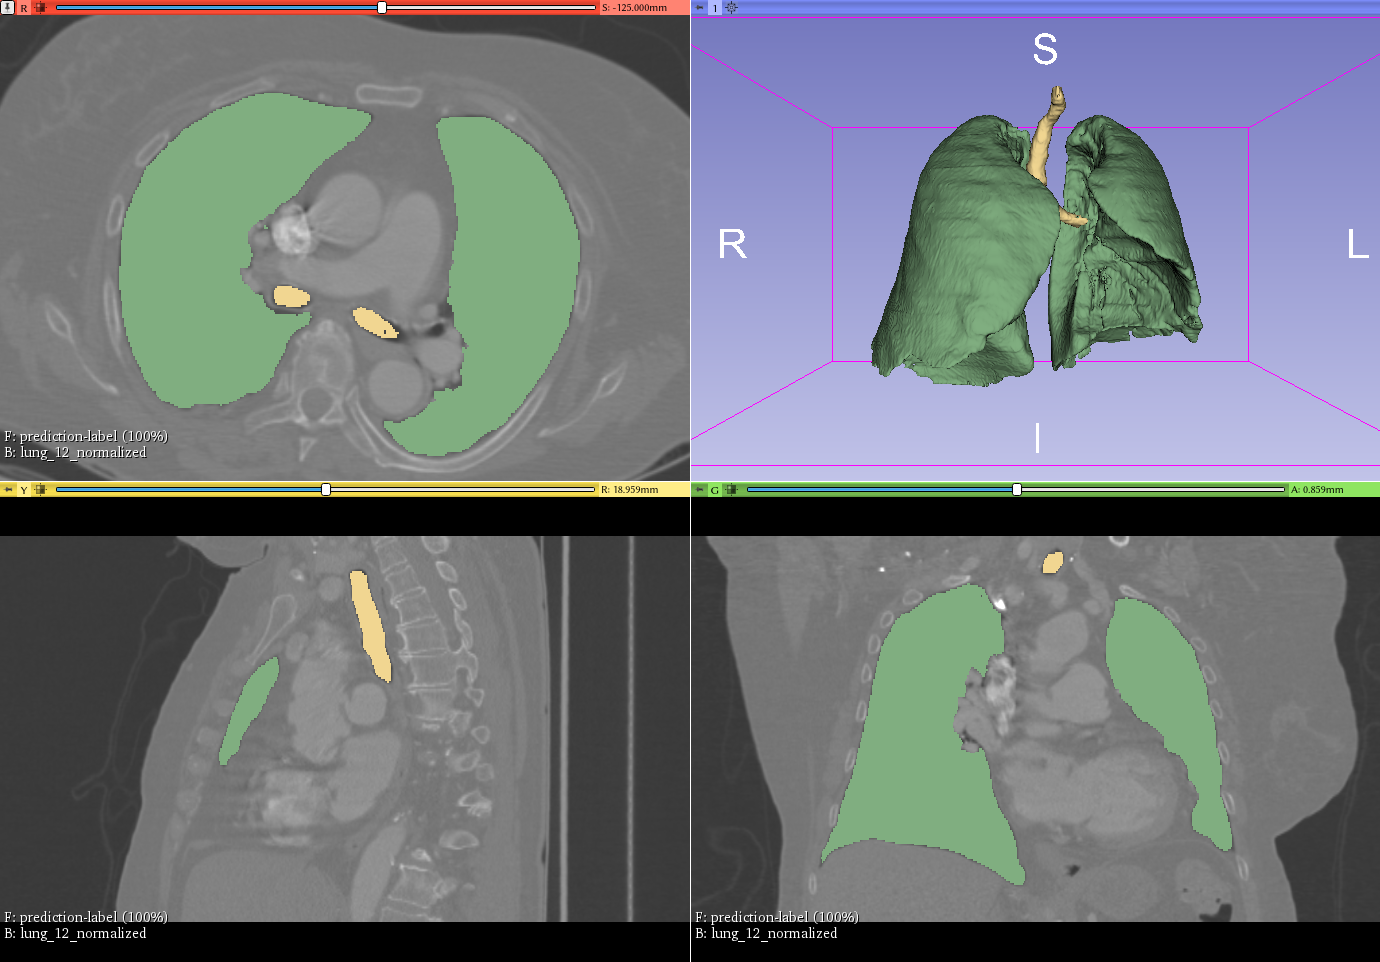
\includegraphics[width=0.49\textwidth, angle=0]{files/Fulllayoutprediction.png}
	\caption{CT scan of the chest with corresponding label map segmentation delineating the lungs (green) and the bronchus (yellow). The first three image portions counterclockwise are the axial, sagittal, and coronal slice views and the final portion is a 3D model of the label.}
	\label{scan_picture}
\end{figure}

The dataset consists of about 10 GB of mhd and raw image files. The files contain a varying number of axial slices of 512 x 512 pixel grey-scale images and corresponding 512 x 512 pixel label maps. Since computational resources were limited a subset of the data was used for this work, more specifically 10 CT image volumes for training and 20 CT image volumes for evaluation were chosen randomly from the set. Furthermore the two label categories for the left and right lungs of the LUNA16 dataset was reduced to one label for the lungs and one label for the bronchus since the two chosen image segmentation CNN architectures were not suitable for representing relative positional information.\newline

\subsection{Preprocessing of image data}
Each raw file was converted to a NIfTI format image file for better processing and visualization. These files each contain a 3D greyscale image volume of a chest CT scan. For more appropriate input values, each image volume was normalized separately following the standard normal distribution ($\mu = 0.0$ and $\sigma = 1.0$).\newline
Then, it was necessary to implement data importation to properly use them. Data from directory was converted into input and label matrices following the size $512$ x $512$ x $n$ with the number of all slices in the dataset $n$.

\subsection{Training and validation}
Both network architectures were trained on the 2145 slices of the 10 training CT scans over 35 epochs.\newline
For the DeepMedic architecture a open-source implementation \cite{deepmediconline} was modified for the purpose of lung segmentation. RMS propagation with a initial learning rate of 0.001 and Nesterov momentum (momentum value of 0.6), and L1 and L2 regularization (0.000001 and 0.0001 respectively) were used. Furthermore, the learning rate was reduced in later epochs in order to improve convergence. For the training a batch size of 10 samples was chosen from the image volumes and the network was evaluated with the binary cross entropy (BCE) as a loss function.\newline
The U-Net architecture was built according to the structure in figure \ref{unetstructure}. For the training process the Adam optimizer with the described loss function $loss = dice loss + BCE$ from chapter \ref{metrics_chapter} was used in combination with a batch size of 3 full 512x512 slices. To get an idea of the performance of the model during training and ensure that only well generalized models were being saved 10\% of the 2145 slices were used for validation while the other 90\% were used for training.\newline

\subsection{Managing the large dataset and image volume size}
Although the dataset was reduced to 10 CT scans some adjustment in the training process still had to be made to handle the size of the dataset and individual 3D image volumes.\newline
Therefore, a generator was defined to reduce the data size that will be fed to the training process at once. The generator feeds batches of images as required to the training process instead of loading the whole dataset onto the GPU and model fitting process at once. Thus reducing the VRAM memory load on the GPU.

\subsection{Prediction, displaying and calculating metrics}

After training the two models were used to predict the segmentation label maps of the 20 test CT scans. The predicted labels were again merged to NIfTI files and displayed. For evaluation an average of the dice loss, the Hausdorff distance and the mean distance were calculated over all 20 test scans.